\documentclass[11pt]{article}

% Change "review" to "final" to generate the final (sometimes called camera-ready) version.
% Change to "preprint" to generate a non-anonymous version with page numbers.
\usepackage[]{acl}
\usepackage{times}
\usepackage{latexsym}

% For proper rendering and hyphenation of words containing Latin characters (including in bib files)
\usepackage[T1]{fontenc}
% For Vietnamese characters
% \usepackage[T5]{fontenc}
% See https://www.latex-project.org/help/documentation/encguide.pdf for other character sets

% This assumes your files are encoded as UTF8
\usepackage[utf8]{inputenc}
\usepackage{microtype}
\usepackage{inconsolata}
\usepackage{graphicx}
\setcitestyle{numbers,square}

% If the title and author information does not fit in the area allocated, uncomment the following
%
%\setlength\titlebox{<dim>}
%
% and set <dim> to something 5cm or larger.

\title{Group X Progress Report:\\My Group's Project Name}


\author{Omar Alam, Sathurshan Arulmohan, Kalp Shah, Jay Sharma \\
  \texttt{\{alamo2,arulmohs,shahk50,sharmj28\}@mcmaster.ca} }

%\author{
%  \textbf{First Author\textsuperscript{1}},
%  \textbf{Second Author\textsuperscript{1,2}},
%  \textbf{Third T. Author\textsuperscript{1}},
%  \textbf{Fourth Author\textsuperscript{1}},
%\\
%  \textbf{Fifth Author\textsuperscript{1,2}},
%  \textbf{Sixth Author\textsuperscript{1}},
%  \textbf{Seventh Author\textsuperscript{1}},
%  \textbf{Eighth Author \textsuperscript{1,2,3,4}},
%\\
%  \textbf{Ninth Author\textsuperscript{1}},
%  \textbf{Tenth Author\textsuperscript{1}},
%  \textbf{Eleventh E. Author\textsuperscript{1,2,3,4,5}},
%  \textbf{Twelfth Author\textsuperscript{1}},
%\\
%  \textbf{Thirteenth Author\textsuperscript{3}},
%  \textbf{Fourteenth F. Author\textsuperscript{2,4}},
%  \textbf{Fifteenth Author\textsuperscript{1}},
%  \textbf{Sixteenth Author\textsuperscript{1}},
%\\
%  \textbf{Seventeenth S. Author\textsuperscript{4,5}},
%  \textbf{Eighteenth Author\textsuperscript{3,4}},
%  \textbf{Nineteenth N. Author\textsuperscript{2,5}},
%  \textbf{Twentieth Author\textsuperscript{1}}
%\\
%\\
%  \textsuperscript{1}Affiliation 1,
%  \textsuperscript{2}Affiliation 2,
%  \textsuperscript{3}Affiliation 3,
%  \textsuperscript{4}Affiliation 4,
%  \textsuperscript{5}Affiliation 5
%\\
%  \small{
%    \textbf{Correspondence:} \href{mailto:email@domain}{email@domain}
%  }
%}

\begin{document}
\maketitle
% \begin{abstract}
% \end{abstract}

\section{Introduction}
Paraphrase detection is the task of determining whether two pieces of text express the same meaning, even if they use different words or sentence structures. This problem is useful in applications such as plagiarism detection, semantic search, duplicate question detection, and large-scale text processing. The task is challenging because surface-level similarity is often misleading: two sentences can share many words but mean different things, while two sentences with very different wording can still be semantically equivalent. As a result, an effective system must go beyond keyword matching and capture the underlying meaning of each sentence in context.

In this project, we study paraphrase detection as a regression problem. Given two tokenized English sentences, the model predicts a score between 0 and 1 that represents how strongly the sentences paraphrase each other. A low score indicates little semantic overlap, while a high score indicates that the two sentences communicate nearly the same idea. To support this task, we use a subset of the ParaNMT-50M dataset, which provides large numbers of sentence pairs with similarity scores. Our overall goal is to build and evaluate models that can learn both word-level similarity and deeper semantic relationships, allowing the system to assign reliable paraphrase scores to unseen sentence pairs.

\section{Related Work}
Past work on paraphrase detection usually looks at the problem in two ways: either deciding if two sentences are paraphrases or giving them a similarity score. One of the best-known datasets in this area is the Microsoft Research Paraphrase Corpus \cite{dolan-brockett-2005}. A closely related area is semantic textual similarity (STS), where the goal is to predict how similar two sentences are on a scale instead of making a yes-or-no decision \cite{cer-etal-2017-semeval}. This is especially relevant to our project because we also treat the problem as score prediction. These works show that paraphrase detection is not just about matching words. Two sentences may use different wording and still mean the same thing.

Another important area of related work is sentence embeddings. Back-translated text has been used to create large paraphrase datasets for learning sentence representations \cite{wieting-etal-2017-learning}. ParaNMT-50M, which we use in this project, builds on that idea \cite{wieting-gimpel-2018-paranmt}. More recent methods use transformer models to create better sentence embeddings. Sentence-BERT made it easier to compare whole sentences using cosine similarity \cite{reimers-gurevych-2019-sentence}, and SimCSE further improved sentence representation quality using contrastive learning \cite{gao-etal-2021-simcse}. No previous paper matches our exact project setup, but these papers are the closest to what we are doing because they focus on paraphrase datasets, similarity scoring, and sentence-level meaning.

\section{Dataset}
We use the ParaNMT-50M dataset for this project. Rather than creating new labels manually, we use the similarity score provided with each sentence pair as the supervision signal for training and evaluation. Each example contains two English sentences and a real-valued score between 0 and 1. Higher scores indicate that the two sentences are more semantically similar, while lower scores indicate weaker similarity. Since our task is formulated as a regression problem, this score is treated as the target value the model must predict.

Each row in the dataset contains three fields: sentence 1, sentence 2, and a score. This format directly matches the paraphrase scoring task because the model receives a pair of sentences as input and learns to predict a continuous similarity label. For example, sentence pairs with almost identical meaning receive scores close to 1.0, while pairs with weaker semantic overlap receive lower scores.

To better understand the labels, we plotted a histogram using the first 1,000,000 rows of the dataset. The x-axis represents paraphrase scores from 0 to 1 using bins of width 0.01, and the y-axis shows the number of sentence pairs in each bin. As shown in Figure~\ref{fig:score-distribution}, the distribution is not uniform. Instead, the dataset is concentrated more heavily toward higher scores, and the largest spike occurs at 1.0. This suggests that highly similar sentence pairs appear much more frequently than weakly related ones in the sampled data.

Because the labels are continuous rather than discrete classes, traditional class balance does not apply directly. However, the score distribution is still clearly imbalanced across the regression range. In particular, the upper score bins contain substantially more examples than many of the lower score bins. This means the dataset is skewed toward highly similar sentence pairs, which may affect model behavior during training and evaluation. For this reason, understanding the label distribution is important when interpreting performance and analyzing prediction errors.

\begin{figure}[t]
    \centering
    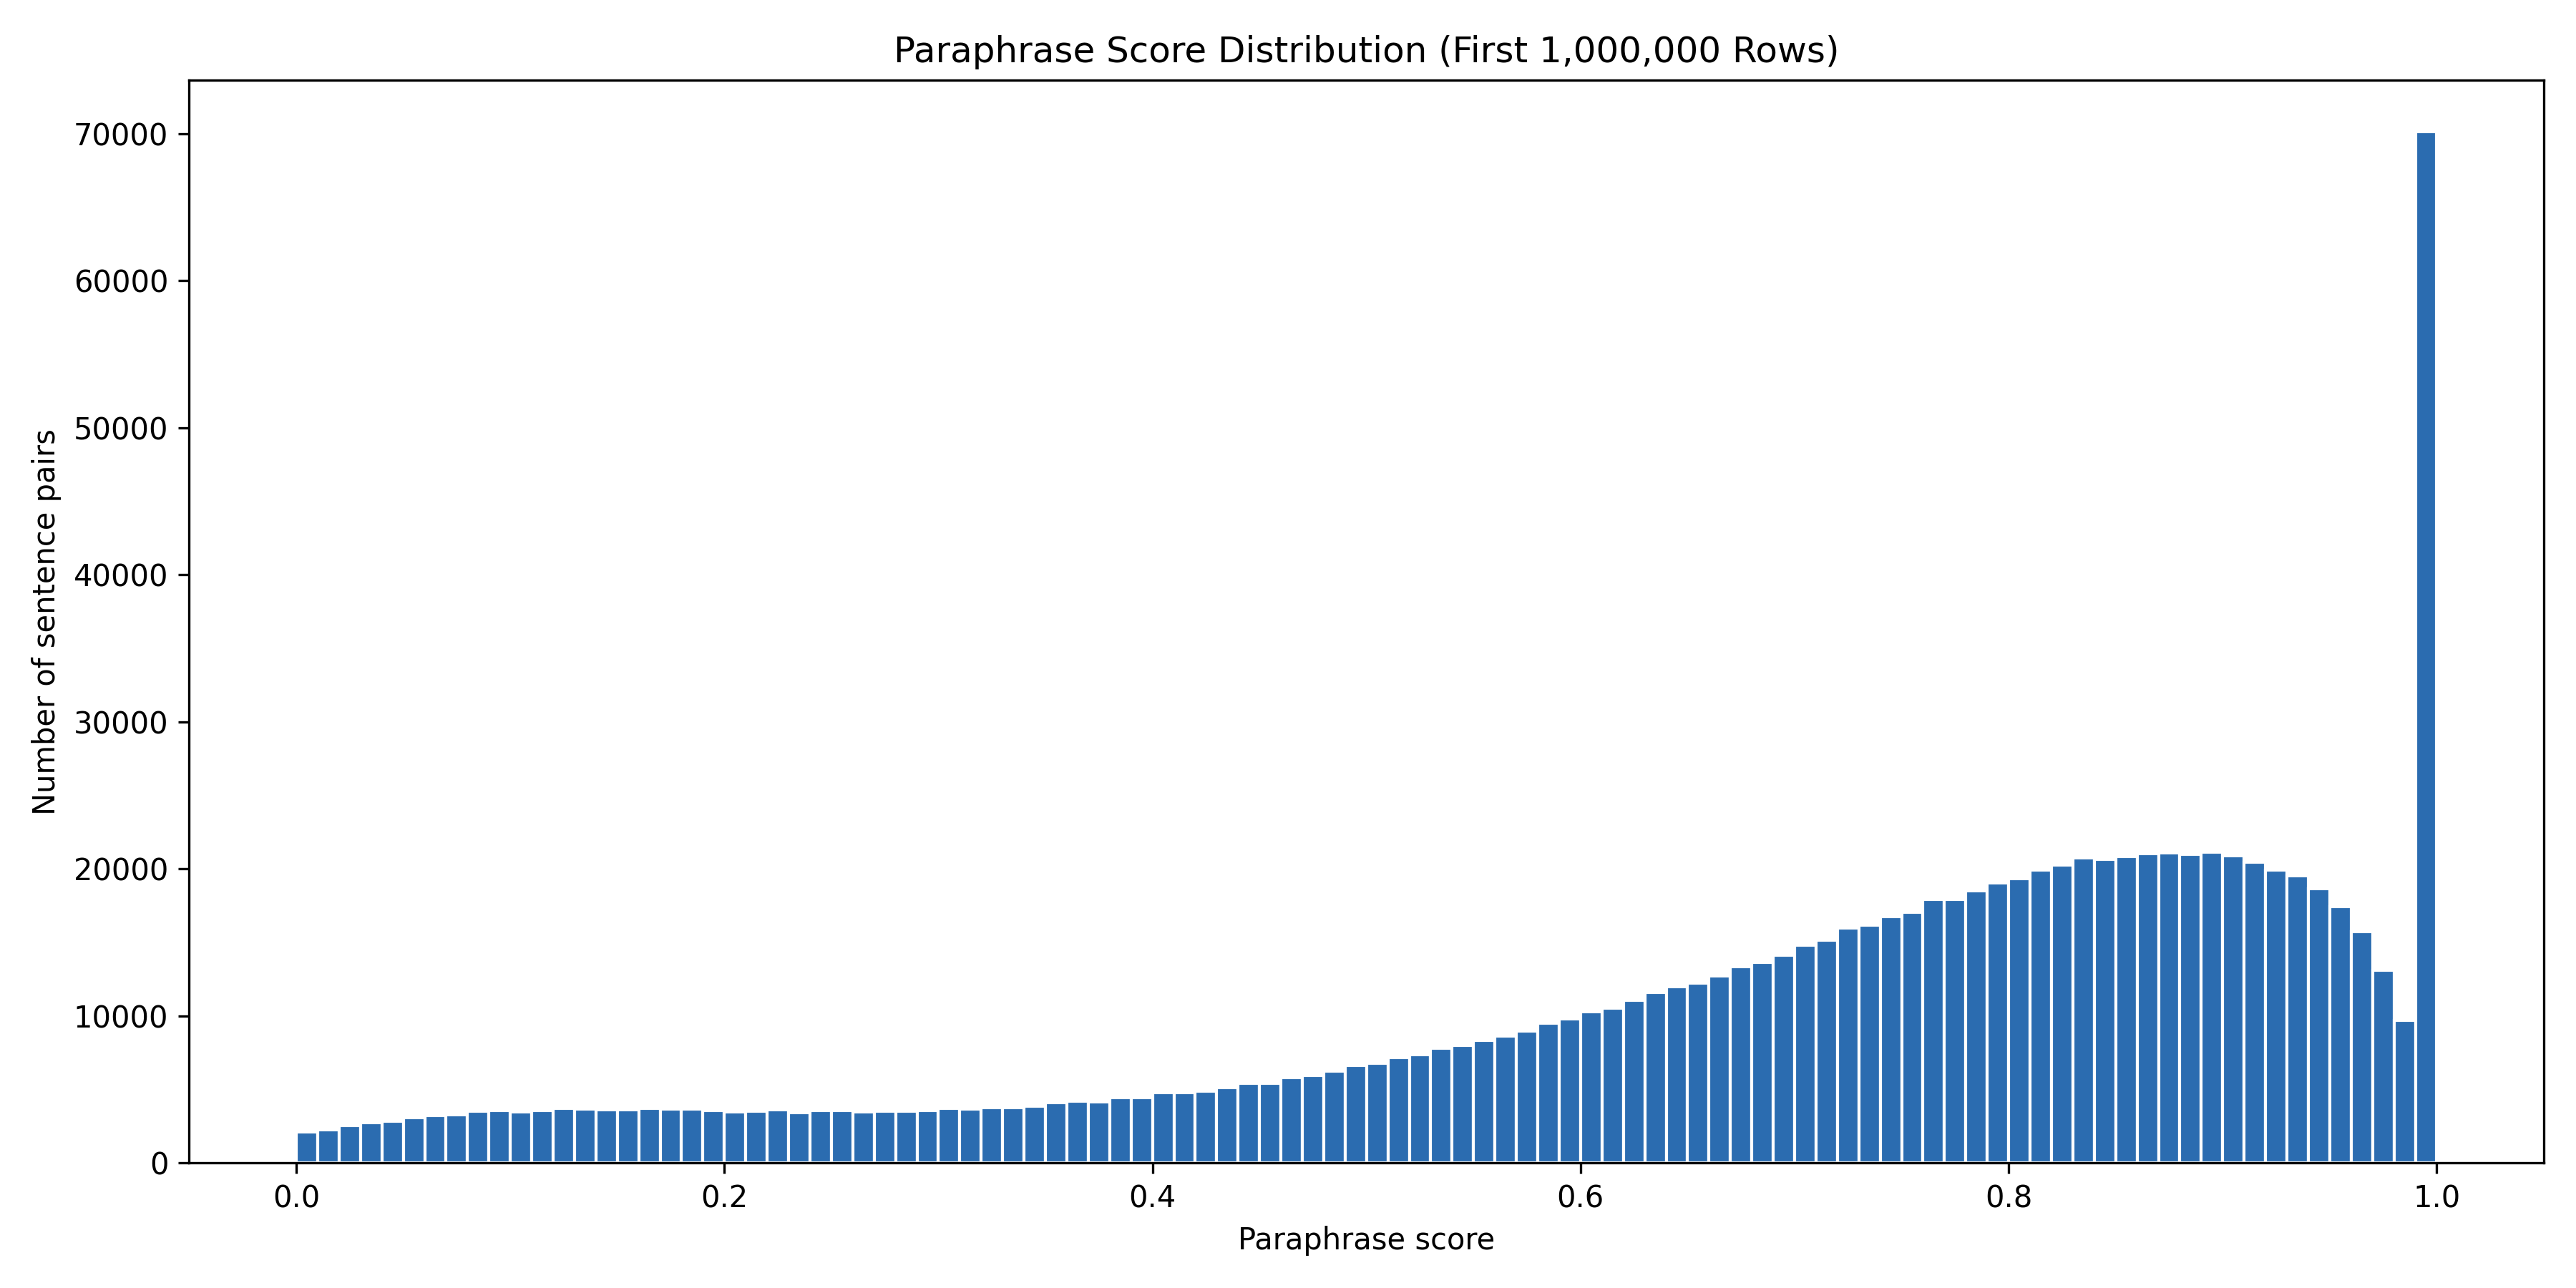
\includegraphics[width=\linewidth]{../score_distribution.png}
    \caption{Distribution of paraphrase scores for the first 1,000,000 rows of ParaNMT-50M.}
    \label{fig:score-distribution}
\end{figure}

\section{Features and Inputs}
Omar

Describe any features you used for your model, or how your data was input to your model. Are you doing feature engineering or feature selection? Are you learning embeddings? Is it all part of one neural network? Refer to item 3. This may range from 0.25 pages to 0.5 pages.

\section{Implementation}

Omar

Describe your model and implementation here. Refer to item 4. This may take around a page.


\section{Evaluation}

Sathurshan

\section{Comparison to Others}

Kalp

\section{Error Analysis}

Sathurshan

What kind of errors are your models making? This doesn't have to be super complicated. Confusion matrices are great. Qualitative observations are also great. This means looking at many cases where your model is wrong (wrong class or high error) and looking for patterns yourself. What about the text might be giving it difficulty? Qualitative analysis is underappreciated and can often give you great insight into issues with your model. Examples are useful here. Refer to item 7. This may be around a half page.

\section{Conclusions}

Summarize your work briefly. Reflect on your implementation and areas for improvement. What do you suggest people work on next (mentioned also in item 7)? This should likely be less than 0.25 pages.

\section*{Team Contributions}

Write in this section a few sentences describing the contributions of each team member. What did each member work on? Refer to item 8.

\begin{thebibliography}{}

\bibitem{dolan-brockett-2005}
W. B. Dolan and C. Brockett, ``Automatically Constructing a Corpus of Sentential Paraphrases,'' in \textit{Proc. Third Int. Workshop on Paraphrasing (IWP2005)}, 2005.

\bibitem{cer-etal-2017-semeval}
D. Cer, M. Diab, E. Agirre, I. Lopez-Gazpio, and L. Specia, ``SemEval-2017 Task 1: Semantic Textual Similarity Multilingual and Crosslingual Focused Evaluation,'' in \textit{Proc. 11th Int. Workshop on Semantic Evaluation (SemEval-2017)}, 2017.

\bibitem{wieting-etal-2017-learning}
J. Wieting, J. Mallinson, and K. Gimpel, ``Learning Paraphrastic Sentence Embeddings from Back-Translated Bitext,'' in \textit{Proc. 2017 Conf. on Empirical Methods in Natural Language Processing}, 2017.

\bibitem{wieting-gimpel-2018-paranmt}
J. Wieting and K. Gimpel, ``ParaNMT-50M: Pushing the Limits of Paraphrastic Sentence Embeddings with Millions of Machine Translations,'' in \textit{Proc. 56th Annual Meeting of the Association for Computational Linguistics}, 2018.

\bibitem{reimers-gurevych-2019-sentence}
N. Reimers and I. Gurevych, ``Sentence-BERT: Sentence Embeddings using Siamese BERT-Networks,'' in \textit{Proc. 2019 Conf. on Empirical Methods in Natural Language Processing and the 9th Int. Joint Conf. on Natural Language Processing}, 2019.

\bibitem{gao-etal-2021-simcse}
T. Gao, X. Yao, and D. Chen, ``SimCSE: Simple Contrastive Learning of Sentence Embeddings,'' in \textit{Proc. 2021 Conf. on Empirical Methods in Natural Language Processing}, 2021.

\end{thebibliography}

% \appendix

% \section{Example Appendix}
% \label{sec:appendix}

% This is an appendix.

\end{document}
